\documentclass[12pt]{article}

\usepackage{amsmath}
\numberwithin{figure}{section}

\usepackage{array}
\usepackage{caption}
\usepackage[top=1in, bottom=1in, left=0.75in, right=0.75in]{geometry}

\usepackage{graphicx}
\graphicspath{{figures/}}

\usepackage[colorlinks=true, allcolors=blue]{hyperref}
\usepackage[utf8]{inputenc}
\usepackage{minted}
\usepackage{multirow}
\usepackage{nameref}
\usepackage{pdfpages}
\usepackage[section]{placeins}

\begin{document}

\begin{titlepage}
  \begin{center} \LARGE
    \vspace*{1.5in}

    ECE 272 Lab 6

    Fall 2018

    \vfill

    Video Graphics Array (VGA)

    Phi Luu

    \vfill

    November 30\textsuperscript{th}, 2018

    Grading TA: Edgar Perez

    Lab Partner: Benjamin Geyer

    \vspace{1.5in}
  \end{center}
\end{titlepage}

%%%%%%%%%%%%%%%%%%%%%%%%%%%%%%%%%%%%%%%%%%%%%%%%%%%%%%%%%%%%%%%%%%%%%%%%%%%%%%%%
% Introduction
%%%%%%%%%%%%%%%%%%%%%%%%%%%%%%%%%%%%%%%%%%%%%%%%%%%%%%%%%%%%%%%%%%%%%%%%%%%%%%%%
\section{Introduction}

\textit{Video graphics array} (\textit{VGA}) is a graphics standard for video display controller first introduced by IBM in 1987. VGA can be used to display a wide range of resolutions and refresh rates. VGA draws on the monitor from left to right and top to bottom. Each pixel is controlled by three analog pins for red, green, and blue (RGB) channels. Although VGA can control a wide range of resolutions and refresh rates, the 640x480 60Hz configuration is commonly used.

For the DE10-Lite, each of the RGB channels is a 4-bit port. The red, green, and blue channels connect to pins 1, 2, and 3 of the VGA connector, respectively. The horizontal sync (hsync) and vertical sync (vsync) signals of the FPGA connect to pins 13 and 14 of the VGA connector, respectively. Hsync and vsync are active-low. When hsync goes to 0, the next line starts to draw; when vsync goes to 0, the drawer goes back to the top of the screen again, starting a new frame. Figure~\ref{fig:de10_lite_vga_pinout}.

\begin{figure}[ht]
  \centering
  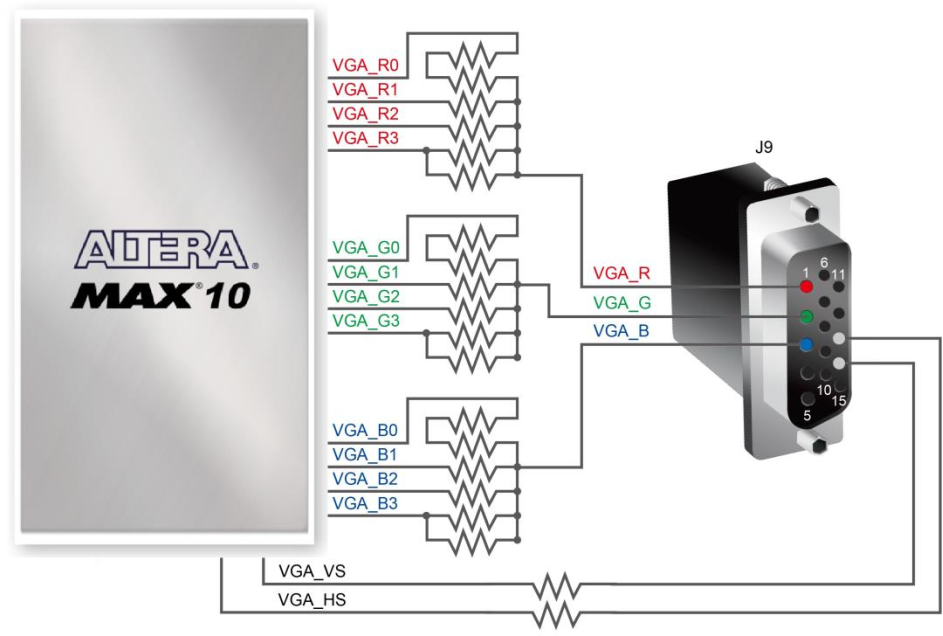
\includegraphics[width=0.75\textwidth]{de10_lite_vga_pinout.png}
  \caption{Connections between the VGA and the MAX 10 FPGA}
  \label{fig:de10_lite_vga_pinout}
\end{figure}

A more detailed pinout of a VGA connector is illustrated by Figure~\ref{fig:vga_connector_pinout}.

\begin{figure}[ht]
  \centering
  \includegraphics[width=0.45\textwidth]{vga_female_socket.png}
  \caption{All 15 pins of a VGA connector. See Table~\ref{tab:vga_pinout_table}.}
  \label{fig:vga_connector_pinout}
\end{figure}

\begin{table}[ht]
  \centering
  \begin{tabular}{ | c | c | l | }
  \hline
  \textbf{Pin} & \textbf{Signal} & \textbf{Description}                                                                     \\ \hline
  1            & RED             & Red video                                                                                \\ \hline
  2            & GREEN           & Green video                                                                              \\ \hline
  3            & BLUE            & Blue video                                                                               \\ \hline
  4            & ID2/RES         & \begin{tabular}[c]{@{}l@{}}formerly Monitor ID bit 2\\ Reserved since E-DDC\end{tabular} \\ \hline
  5            & GND             & Ground (H-Sync)                                                                          \\ \hline
  6            & RED\_RTN        & Red return                                                                               \\ \hline
  7            & GREEN\_RTN      & Green return                                                                             \\ \hline
  8            & BLUE\_RTN       & Blue return                                                                              \\ \hline
  9            & KEY/PWR         & \begin{tabular}[c]{@{}l@{}}formerly key\\ now +5V DC\end{tabular}                        \\ \hline
  10           & GND             & Ground (V-Sync, DDC)                                                                     \\ \hline
  11           & ID0/RES         & \begin{tabular}[c]{@{}l@{}}formerly Monitor ID bit 0\\ reserved since E-DDC\end{tabular} \\ \hline
  12           & ID1/SDA         & \begin{tabular}[c]{@{}l@{}}formerly Monitor ID bit 1\\ PC data since DDC2\end{tabular}   \\ \hline
  13           & HSync           & Horizontal sync                                                                          \\ \hline
  14           & VSync           & Vertical sync                                                                            \\ \hline
  15           & ID3/SCL         & \begin{tabular}[c]{@{}l@{}}formerly Monitor ID bit 3\\ I2C clock since DDC2\end{tabular} \\ \hline
  \end{tabular}
  \caption{VGA pinout}
  \label{tab:vga_pinout_table}
\end{table}

%%%%%%%%%%%%%%%%%%%%%%%%%%%%%%%%%%%%%%%%%%%%%%%%%%%%%%%%%%%%%%%%%%%%%%%%%%%%%%%%
% Design
%%%%%%%%%%%%%%%%%%%%%%%%%%%%%%%%%%%%%%%%%%%%%%%%%%%%%%%%%%%%%%%%%%%%%%%%%%%%%%%%
\section{Design}

The timing sequence of an VGA controller is as follows: the pixels are displayed from left to right and top to bottom. When all the pixels of the active resolution are displayed, there is a blank period called the \textit{front porch} which signaling the start of a \textit{sync pulse}. When the front porch period finishes, the sync pulse itself is toggled from HIGH to LOW (the sync pulses are active-low). This sync pulse signals the "reset" of the xy counter: the hsync pulse resets the xy counter to the left most of the next line, whereas the vsync pulse resets the xy counter to the top left of the screen. After sync pulse period finishes, the sync pulse is toggled back to HIGH for a period of time called the \textit{back porch}.

Figure~\ref{fig:640x480_60hz_vga_timing_sequence} shows the VGA timing sequence for the 640x480 resolution with 60 Hz refresh rate.

\begin{figure}[ht]
  \centering
  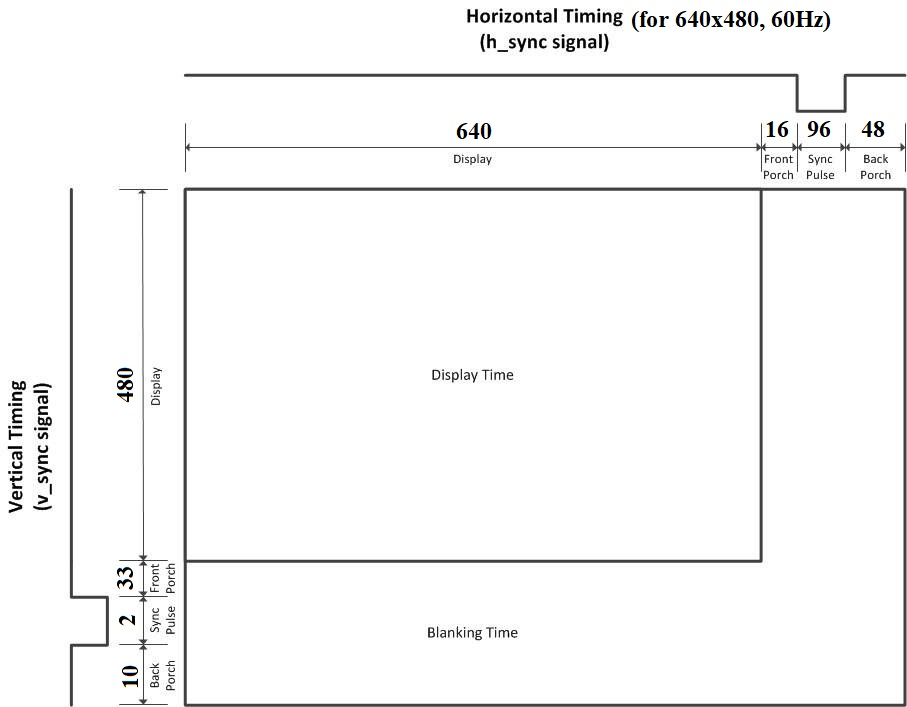
\includegraphics[width=\textwidth]{vga_timing_sequence_640x480_60hz.png}
  \caption{The display, front porch, sync pulse, and back porch signals of the horizontal timing and vertical timing of 640x480 60Hz monitor}
  \label{fig:640x480_60hz_vga_timing_sequence}
\end{figure}

\begin{figure}[ht]
  \centering
  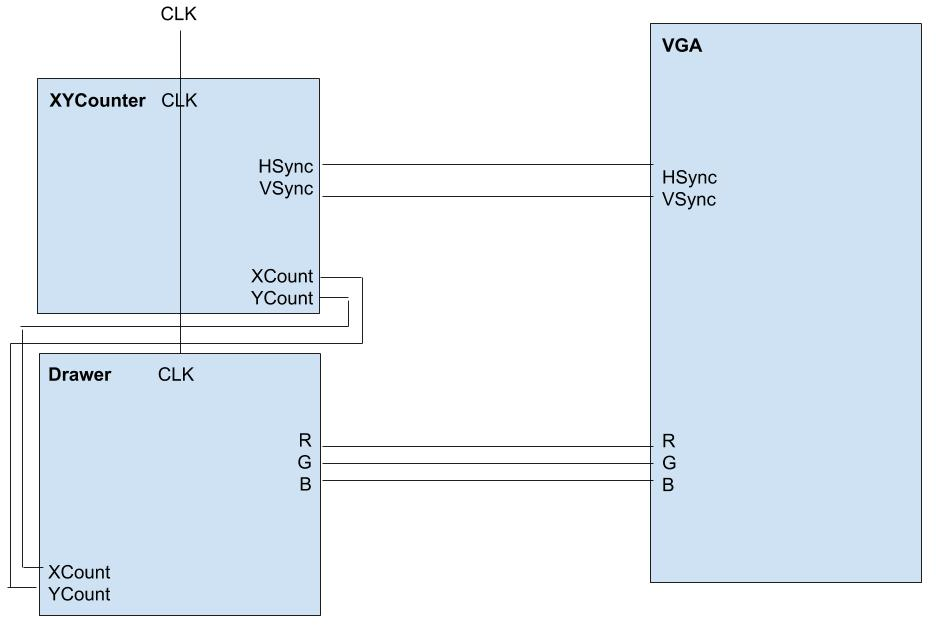
\includegraphics[width=\textwidth]{lab6_block_diagram.png}
  \caption{The block diagram}
  \label{fig:block_diagram}
\end{figure}

%%%%%%%%%%%%%%%%%%%%%%%%%%%%%%%%%%%%%%%%%%%%%%%%%%%%%%%%%%%%%%%%%%%%%%%%%%%%%%%%
% Experiment Notes
%%%%%%%%%%%%%%%%%%%%%%%%%%%%%%%%%%%%%%%%%%%%%%%%%%%%%%%%%%%%%%%%%%%%%%%%%%%%%%%%
\section{Experiment Notes}

%%%%%%%%%%%%%%%%%%%%%%%%%%%%%%%%%%%%%%%%
% Reflection
%%%%%%%%%%%%%%%%%%%%%%%%%%%%%%%%%%%%%%%%
\subsection*{Reflection}

%%%%%%%%%%%%%%%%%%%%%%%%%%%%%%%%%%%%%%%%
% Study Questions
%%%%%%%%%%%%%%%%%%%%%%%%%%%%%%%%%%%%%%%%
\subsection*{Study Questions}

\begin{enumerate}
  \item What was the toughest aspect of ECE 272? What should be changed or added to the ECE 272 manual to make this course better?



  \item What would you like to explore further about Lattice Diamond or Digital Logic Design?



  \item What section of ECE 272 did you dislike the most? Why?



  \item What was your favorite section of ECE 272? Why?


\end{enumerate}

%%%%%%%%%%%%%%%%%%%%%%%%%%%%%%%%%%%%%%%%%%%%%%%%%%%%%%%%%%%%%%%%%%%%%%%%%%%%%%%%
% Appendix
%%%%%%%%%%%%%%%%%%%%%%%%%%%%%%%%%%%%%%%%%%%%%%%%%%%%%%%%%%%%%%%%%%%%%%%%%%%%%%%%
\section*{Appendix} \label{sec:appendix}

\begin{center}
  \textbf{VgaTopLevel.qsf} (Pin Assignment)
\end{center}

\inputminted[breaklines, firstline=38, fontfamily=tt, fontsize=\small, frame=lines, framesep=1.5em, linenos, numbersep=1.5em, style=vs]{text}{lab6/VgaTopLevel.qsf}

\begin{center}
  \textbf{VgaTopLevel.sv}
\end{center}

\inputminted[breaklines, fontfamily=tt, fontsize=\small, frame=lines, framesep=1.5em, linenos, numbersep=1.5em, style=vs]{systemverilog}{lab6/VgaTopLevel.sv}

\begin{center}
  \textbf{HalfClock.sv}
\end{center}

\inputminted[breaklines, fontfamily=tt, fontsize=\small, frame=lines, framesep=1.5em, linenos, numbersep=1.5em, style=vs]{systemverilog}{lab6/HalfClock.sv}

\begin{center}
  \textbf{VgaController.sv}
\end{center}

\inputminted[breaklines, fontfamily=tt, fontsize=\small, frame=lines, framesep=1.5em, linenos, numbersep=1.5em, style=vs]{systemverilog}{lab6/VgaController.sv}

\begin{center}
  \textbf{VgaDrawer.sv}
\end{center}

\inputminted[breaklines, fontfamily=tt, fontsize=\small, frame=lines, framesep=1.5em, linenos, numbersep=1.5em, style=vs]{systemverilog}{lab6/VgaDrawer.sv}

%%%%%%%%%%%%%%%%%%%%%%%%%%%%%%%%%%%%%%%%%%%%%%%%%%%%%%%%%%%%%%%%%%%%%%%%%%%%%%%%
% % Bibliography
% %%%%%%%%%%%%%%%%%%%%%%%%%%%%%%%%%%%%%%%%%%%%%%%%%%%%%%%%%%%%%%%%%%%%%%%%%%%%%%%%
% \bibliographystyle{ieeetr}
% \bibliography{references}

\end{document}
